\documentclass[a4]{article}

\usepackage[left=3cm,right=3cm,top=2cm,bottom=2cm]{geometry} 

\usepackage[utf8]{inputenc}   % otra alternativa para los caracteres acentuados y la "ñ"
\usepackage[           spanish % para poder usar el español
                      ,es-tabla % para los captions de las tablas
                       ]{babel}   
%\decimalpoint %para usar el punto decimal en vez de coma para los números con decimales

\usepackage[T1]{fontenc}
\usepackage{lmodern}

\usepackage{parskip}
\usepackage{xcolor}

\usepackage{caption}
\usepackage{hyperref}
\usepackage{enumerate} % paquete para poder personalizar fácilmente la apariencia de las listas enumerativas
\usepackage{listings}
\usepackage{xcolor}
\usepackage{amsmath}
\definecolor{codegreen}{rgb}{0,0.6,0}
\definecolor{codegray}{rgb}{0.2,0.2,0.2}
\definecolor{codepurple}{rgb}{0.58,0,0.82}
\definecolor{backcolour}{rgb}{0.95,0.95,0.92}

\lstdefinestyle{mystyle}{
	backgroundcolor=\color{backcolour},   
	commentstyle=\color{codegray},
	keywordstyle=\color{codegreen},
	numberstyle=\tiny\color{blue},
	stringstyle=\color{red},
	basicstyle=\ttfamily\normalsize,
	breakatwhitespace=false,         
	breaklines=true,                 
	captionpos=b,                    
	keepspaces=true,                 
	numbers=left,                    
	numbersep=5pt,                  
	showspaces=false,                
	showstringspaces=false,
	showtabs=false,                  
	tabsize=2
}

\lstset{style=mystyle}
\usepackage{graphicx} % figuras
\usepackage{subfigure} % subfiguras

\usepackage{amsfonts}
\usepackage{amsmath}

\definecolor{gris}{RGB}{220,220,220}
	
\usepackage{float} % para controlar la situación de los entornos flotantes

\restylefloat{figure}
\restylefloat{table} 

\newcommand{\HRule}{\rule{\linewidth}{0.5mm}}

\author{Pilar Navarro Ramírez}
\date{\vspace{-5mm}}

\title{\huge APRENDIZAJE AUTOMÁTICO: Práctica 2 \HRule\vspace{-4mm}}

\begin{document}
\maketitle
\tableofcontents

\newpage

\section{Ejercicio sobre la complejidad de H y el ruido}

\textbf{En este ejercicio debemos aprender la dificultad que introduce la aparición de ruido en las
etiquetas a la hora de elegir la clase de funciones más adecuada.}

\subsection{Ejercicio 1}
\textbf{Dibujar gráficas con las nubes de puntos simuladas con las siguientes condiciones:}

\textbf{a) Considere N = 50, dim = 2, rango = [-50, +50] con \lstinline|simula_unif (N, dim, rango)|.}

\textbf{b) Considere N = 50, dim = 2 y sigma = [5, 7] con \lstinline|simula_gaus(N, dim, sigma)|.}

Haciendo uso de la función \lstinline|simula_unif (N, dim, rango)|, tal y como nos dice el enunciado, generamos una muestra en dimensión 2 de 50 puntos uniformemente distribuidos en el cuadrado \\ $ [-50, +50]\times [-50, +50] $. A continuación, visualizamos dicha muestra con la función \lstinline|scatter| de \lstinline|matplotlib| y obtenemos lo siguiente:
\begin{figure}[H]
	\centering
	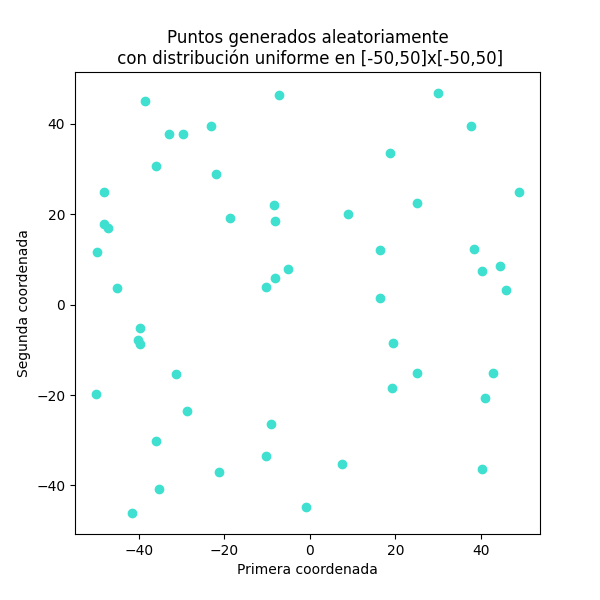
\includegraphics[width=0.6\linewidth]{img/Figure_1}
	\caption{}
	\label{fig:figure1}
\end{figure}
Si repetimos el proceso, pero en este caso usando la función \lstinline|simula_gaus(N, dim, sigma)| para generar 50 puntos de una distribución normal con media 0 y varianza 5 para la primera coordenada y 7 para la segunda (desviaciones típicas $\sqrt{5}$ y $ \sqrt{7} $), tenemos la siguiente nube de puntos:
\begin{figure}[H]
	\centering
	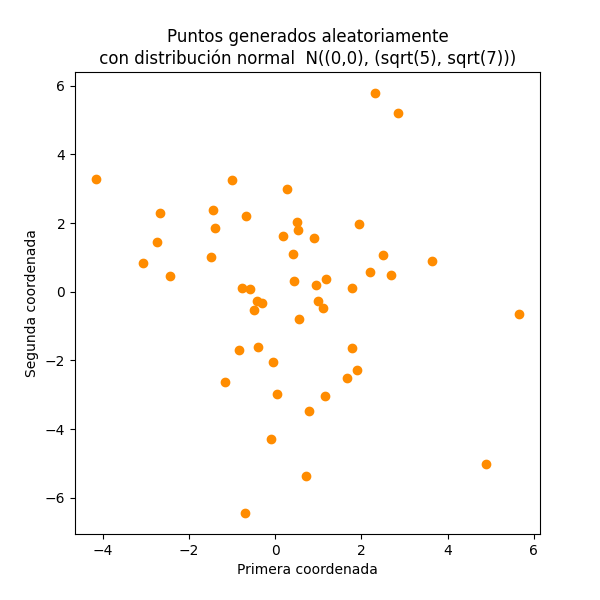
\includegraphics[width=0.6\linewidth]{img/Figure_2}
	\caption{}
	\label{fig:figure2}
\end{figure}
Representamos las dos muestras juntas:
\begin{figure}[H]
	\centering
	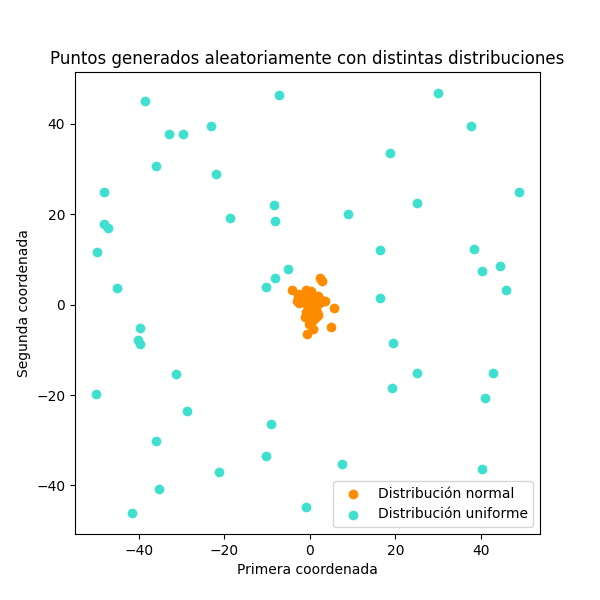
\includegraphics[width=0.6\linewidth]{img/Figure_3}
	\caption{}
	\label{fig:figure3}
\end{figure}
Nos damos cuenta de que la primera muestra está efectivamente distribuida de manera uniforme en el cuadrado, mientras que la segunda está concentrada entorno al punto (0,0), pues esta es la media de la distribución que sigue dicha muestra, siendo la dispersión de los puntos en la segunda coordenada mayor que en la primera por ser la varianza en esta dimensión mayor (7 frente a 5).

\subsection{Ejercicio 2}
\textbf{Vamos a valorar la influencia del ruido en la selección de la complejidad de la clase
de funciones. Con ayuda de la función \lstinline|simula_unif (100, 2, [-50, 50])| generamos una
muestra de puntos 2D a los que vamos a añadir una etiqueta usando el signo de la función
$ f (x, y) = y - ax - b $, es decir, el signo de la distancia de cada punto a la recta simulada con
\lstinline|simula_recta()|.}

Como en el ejercicio anterior, generamos una muestra uniforme en el cuadrado $ [-50, +50]\times [-50, +50] $ de 100 puntos 2D usando la función \lstinline|simula_unif|. Generamos también los parámetros a y b de una recta que corta al cuadrado, con la función \lstinline|simula_recta|. Los parámetros aleatorios obtenidos en mi ejecución con semilla de 1 han sido $ a:  -0.6771584922002485,  b: -18.89022818933684 $. 

Usamos la recta obtenida para etiquetar los puntos de la muestra. Para ello, consideramos la función $ f (x, y) = y - ax - b $, de manera que la etiqueta de un punto (x,y) será el signo de $ f (x, y)$. Esto es, la etiqueta del punto será +1 si este queda por encima de la recta $y=ax+b$, o justo en ella, y -1 si queda por debajo. 

 La función \lstinline|etiquetar(x,f,ruido)| se encarga de etiquetar los puntos de la muestra x según el signo de la función f pasada como parámetro. Además, añade ruido en el etiquetado si el parámetro \textit{ruido} es \lstinline|True| (para más detalles ver el código). Así, haremos uso de dicha función con $ f (x, y) = y - ax - b $ para etiquetar la muestra como hemos descrito.


\subsubsection{Apartado a)}
\textbf{Dibujar un gráfico 2D donde los puntos muestren el resultado de su etiqueta. Dibuje también la recta usada para etiquetar.}

Para representar la muestra junto con la frontera de clasificación f (en este caso nuestra recta) hemos implementado la función \lstinline|plotEtiquetado(x,etiquetas,f,args)|. Al ejecutarla para nuestra muestra uniforme y el etiquetado considerado obtenemos:

\begin{figure}[H]
	\centering
	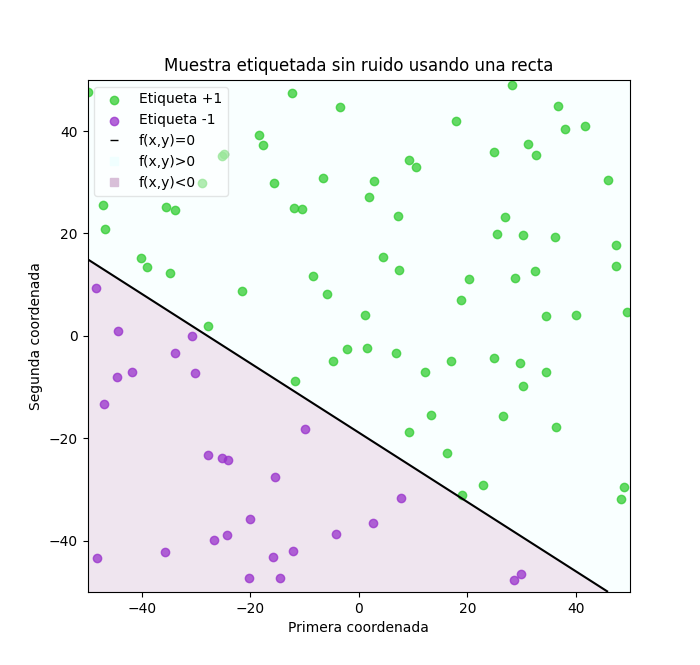
\includegraphics[width=0.65\linewidth]{img/Figure_4}
	\caption{}
	\label{fig:figure4}
\end{figure}


Podemos ver que todos los puntos están correctamente clasificados respecto de la recta, pues hemos usado precisamente esa recta para etiquetar los puntos. 

\subsubsection{Apartado b)}

\textbf{Modifique de forma aleatoria un 10\% de las etiquetas positivas y otro
10\% de las negativas y guarde los puntos con sus nuevas etiquetas. Dibuje de nuevo
la gráfica anterior.}

Volvemos a generar el etiquetado con la función \lstinline|etiquetar|, pero en este caso con el parámetro ruido a \lstinline|True|, de modo que se cambia el signo  del 10\% de las etiquetas de cada clase. Visualizamos de nuevo el resultado, con \lstinline|plotEtiquetado|:

\begin{figure}[H]
	\centering
	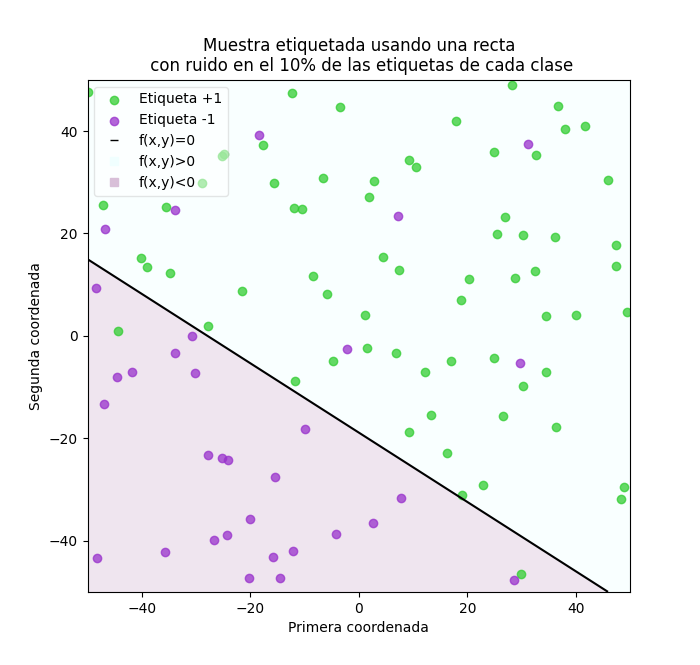
\includegraphics[width=0.65\linewidth]{img/recta_ruido}
	\caption{}
	\label{fig:recta_ruido}
\end{figure}

Nos damos cuenta de que, debido al ruido, ahora hay puntos que están mal clasificados con respecto a la recta. 

Consideramos la función \lstinline|Error(x,etiquetas,f)|, que cuenta la proporción de puntos de la muestra x que la frontera de clasificación determinada por la función f clasifica incorrectamente. Concretamente, calcula el siguiente valor:
$$Error=\frac{1}{N}\sum_{i=1}^{N}[[sign(f(x[i])\neq etiquetas[i])]]$$ donde N es el tamaño de la muestra x, x[i] es el punto i-ésimo de la muestra y etiquetas[i] el valor de su etiqueta. 

Calculamos este error para la muestra etiquetada con ruido y la recta de clasificación considerada, $f(x,y)=y-ax-b$, y obtenemos un valor de 0.09, que era más o menos lo esperado, pues debería haber un 10\% de los puntos mal clasificados (0.1) al introducir el ruido. 
\newpage
\subsubsection{Apartado c)}

\textbf{Supongamos ahora que las siguientes funciones definen la frontera de
clasificación de los puntos de la muestra en lugar de una recta:}
\begin{itemize}
	\item $ f (x, y) = (x - 10)^2 + (y - 20)^2 - 400 $
	\item $ f (x, y) = 0,5(x + 10)^2 + (y - 20)^2 - 400 $
	\item $ f (x, y) = 0,5(x - 10)^2 - (y + 20)^2 - 400 $
	\item $ f (x, y) = y - 20x^2 - 5x + 3 $
\end{itemize}
\textbf{Visualizar el etiquetado generado en 2b junto con cada una de las gráficas de cada
una de las funciones. Comparar las regiones positivas y negativas de estas nuevas
funciones con las obtenidas en el caso de la recta. Argumente si estas funciones más
complejas son mejores clasificadores que la función lineal. Observe las gráficas y diga
que consecuencias extrae sobre la influencia del proceso de modificación de etiquetas
en el proceso de aprendizaje. Explicar el razonamiento.}

Etiquetamos en este caso la muestra con cada una de las nuevas funciones que nos dan, utilizando la función \lstinline|etiquetar| con \lstinline|ruido=True|, y representamos gráficamente el etiquetado generado junto con la frontera de clasificación usando \lstinline|plotEtiquetado|:

\begin{figure}[H]
	\centering    
	\subfigure[$(x - 10)^2 + (y - 20)^2 - 400 $; Error=0.07]{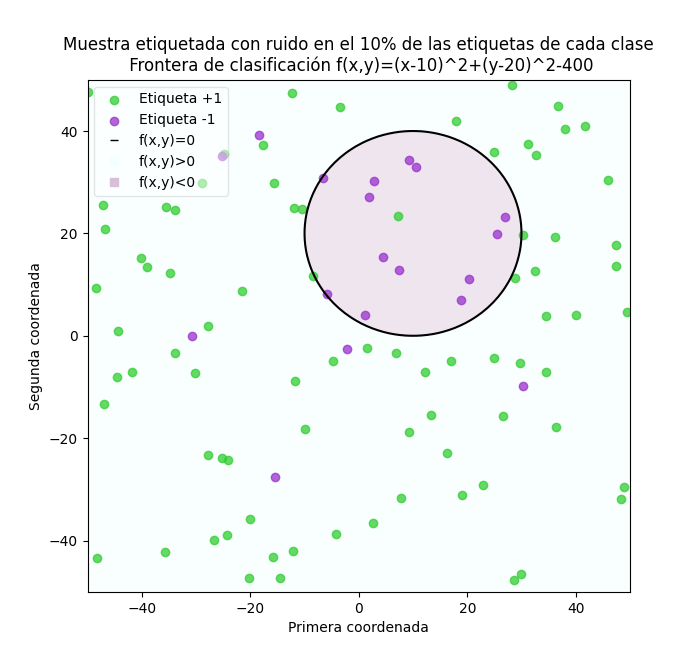
\includegraphics[width=77mm]{img/f1.png}}
	\subfigure[$0,5(x + 10)^2 + (y - 20)^2 - 400 $; Error=0.09]{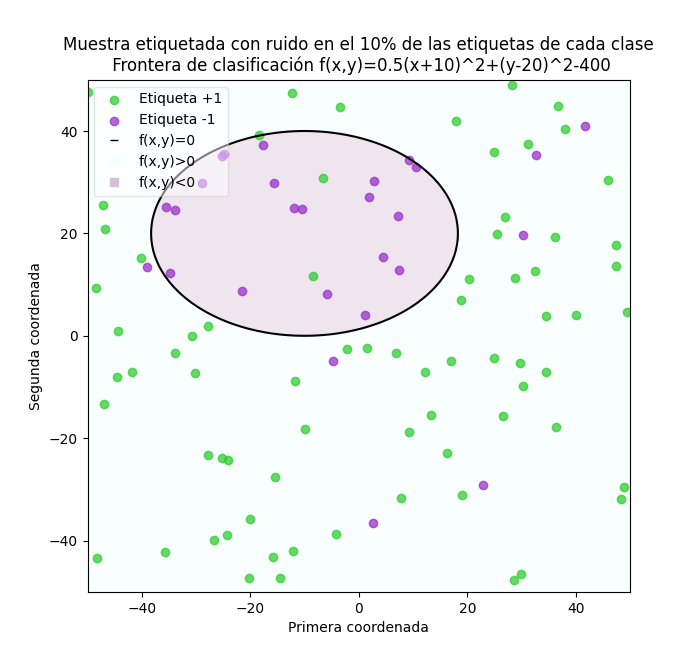
\includegraphics[width=77mm]{img/f2.png}}
	\caption{}
	\label{fig:fronteras1}
\end{figure}

\begin{figure}[H]
	\centering    
	\subfigure[$ 0,5(x - 10)^2 - (y + 20)^2 - 400 $; Error=0.09]{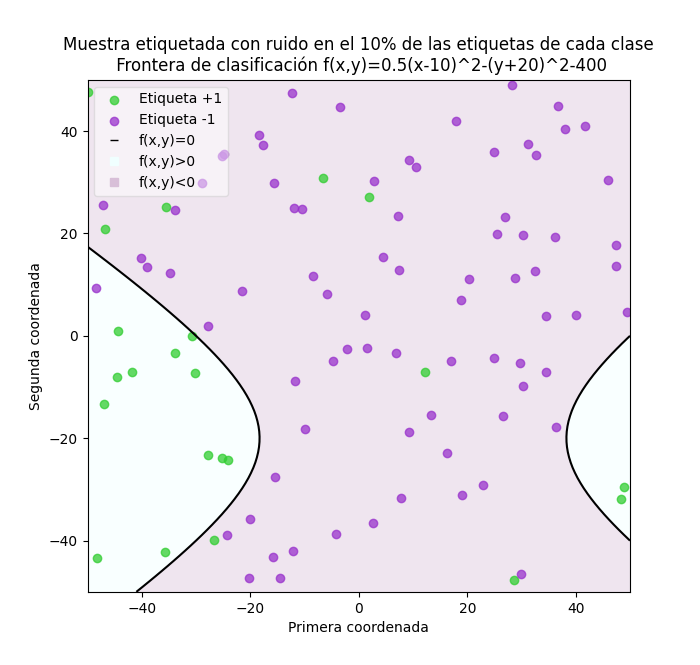
\includegraphics[width=77mm]{img/f3.png}}
	\subfigure[$ y - 20x^2 - 5x + 3 $; Error=0.08]{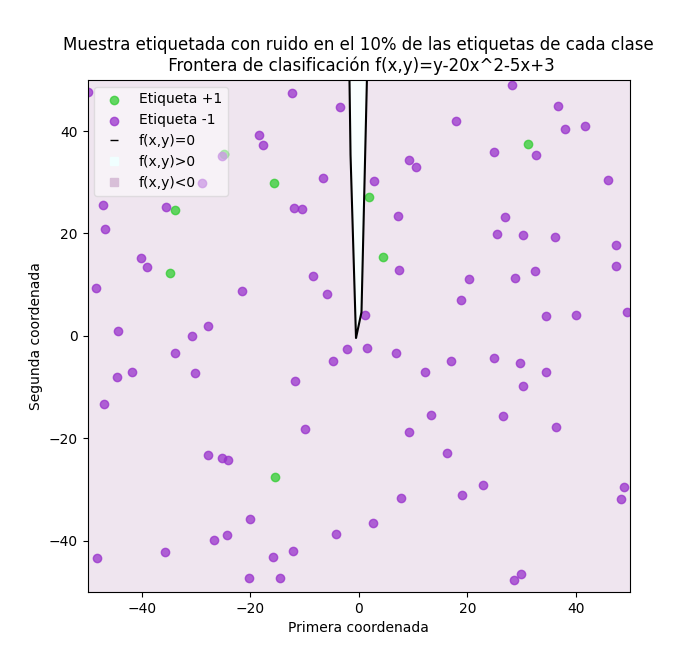
\includegraphics[width=77mm]{img/f4.png}}
	\caption{}
	\label{fig:fronteras2}
\end{figure}

El error ha sido obtenido usando la función \lstinline|Error(x,etiquetas,f)|, con el clasificador f y las etiquetas correspondientes en cada caso. 

La forma de las regiones positivas y negativas dependen de la función f considerada, podemos ver que es diferente en cada uno de los casos. Dependiendo de los datos, de cómo sean las regiones positiva y negativa, será mejor una frontera de clasificación u otra. 

En todos los casos el error cometido por los clasificadores es aproximadamente del 10\%, como era de esperar al modificar las etiquetas del 10\% de los puntos.  Así, ninguna de las funciones es mejor clasificadora que otra, todas clasifican igual de bien, pues en todos los casos la función ha sido empleada para generar el etiquetado correspondiente y se ha introducido el mismo porcentaje de ruido. 

El hecho de que una función sea más compleja no hace que la clasificación sea mejor o peor, sino que depende de cómo de bien se ajuste dicha función a los datos del problema concreto. 

Vemos que el ruido afecta por igual en todos los casos, aproximadamente el 10\% de los puntos son clasificados incorrectamente siempre. Aunque la frontera de clasificación sea la adecuada y se ajuste bien a los datos, no va a poder clasificar correctamente los puntos con ruido. 

En algunas circunstancias es posible que una clase de funciones más compleja consiga clasificar correctamente casi todos los puntos, incluso los datos con ruido, de lo que no sería capaz una función simple. Sin embargo, esto haría que se produzca un sobreajuste a los datos de la muestra, por lo que la clasificación no generalizaría bien fuera de la muestra, es decir, el error en la muestra sería muy bajo pero el error fuera de la muestra sería grande. En nuestro estudio esto no ocurre, pues el porcentaje de ruido introducido es pequeño.

\newpage
\section{Modelos lineales}
\subsection{Ejercicio 1: Algoritmo perceptron}

\textbf{Implementar la función \lstinline|ajusta_PLA(datos, label, max_iter, vini)|
que calcula el hiperplano solución a un problema de clasificación binaria usando el
algoritmo PLA.}

El algoritmo PLA (\textit{Perceptron Learning Algorithm}) es un caso particular de SGD (ver práctica 1), donde el tamaño de batch y la tasa de aprendizaje son 1, y el error a minimizar es $\frac{1}{N}\sum_{n=1}^{N}[[sign(w^Tx_n)\neq y_n)]]$ ($x_n$ es el punto n-ésimo de la muestra, $y_n$ es su etiqueta, N es el número de datos en la muestra y w es el vector de pesos que determina una función lineal), que es el error usado en clasificación lineal. La función \lstinline|Error(x,etiquetas,w)| implementa este error.

El gradiente del error en un punto $(x_n,y_n)$ es 0 si $sign(w^Tx_n)=y_n $ y $-y_nx_n$ si $sign(w^Tx_n)\neq y_n $. 

Por tanto, lo que hace PLA es recorrer varias veces (hasta un máximo número de iteraciones especificado por el programador) uno por uno los datos $(x_n,y_n)$ de la muestra, comprobando si $sign(w^Tx_n)=y_n $, es decir, mirando si el dato está o no bien clasificado con respecto a la solución $ w $ obtenida hasta ese momento. En caso de que el dato esté bien clasificado el vector w no sufre ninguna modificación. En caso contrario se le suma a este $y_nx_n$, es decir, se actualiza el vector de pesos en la dirección del gradiente descendente del error en ese punto. El algoritmo para cuando se alcanza el número de iteraciones máximo o cuando se recorre todo el conjunto de datos y no se encuentra ningún punto mal clasificado (no se modifica w en un pase completo por el conjunto de datos). Así, el algoritmo PLA queda como sigue:

\begin{lstlisting}[language=Python]
PLA:
w <-- vini  # Vector inicial de pesos
cambio <-- True
iteraciones <-- 0
while cambio and iteraciones<max_iteraciones:
	cambio <-- False
	for x in datos:
		if signo(w.T*x)!= y: # Etiqueta asociada al punto x
			w <-- w + x*y
			change <-- True
	iteraciones <-- iteraciones + 1
return w, iteraciones

\end{lstlisting}

Este algoritmo está implementado por la función \lstinline|ajusta_PLA(datos, label, max_iter, vini)|. 


\subsubsection{Apartado a)}
  
\textbf{Ejecutar el algoritmo PLA con los datos simulados en los apartados 2a) de la
sección 1. Inicializar el algoritmo con: a) el vector cero y, b) con vectores de
números aleatorios en $ [0, 1] $ (10 veces). Anotar el número medio de iteraciones
necesarias en ambos para converger. Valorar el resultado relacionando el punto
de inicio con el número de iteraciones.
}

Implementamos la función \lstinline|iteracionesPLA(x, etiquetas)| que ejecuta el algoritmo PLA tal y como se describe en el enunciado. Ejecuta PLA sobre la muestra etiquetada que se le pasa como parámetro (\textbf{x} es el conjunto de puntos de la muestra y \textbf{etiquetas} es el vector de etiquetas asociado a la muestra x) con \lstinline|vini| igual al vector (0,0,0), calcula el error asociado a la solución obtenida con la función \lstinline|Error(x,etiquetas,w)|, visualiza la muestra junto con el hiperplano solución e imprime el número de iteraciones que necesitó el algoritmo para encontrar la solución. A continuación repite el proceso 10 veces pero partiendo en cada repetición de un vector aleatorio con valores en $ [0, 1] $ y calcula el número medio de iteraciones necesarias en las 10 repeticiones así como el error medio. 

Ejecutamos \lstinline|iteracionesPLA(x, etiquetas)| con la muestra y etiquetas generadas en el apartado 2a) de la sección 1 (sin ruido) y los resultados obtenidos han sido los siguientes:

\begin{table}[H]
	\begin{center}
	\begin{tabular}{|c|c|c|}
		\hline
		\textbf{Vector inicial de pesos} & \textbf{Número de iteraciones } & \textbf{Error} \\ \hline
		[0,0,0] & 75 & 0 \\ \hline
		[ 0.48432, 0.65005 0.14394 ] & 69 & 0 \\ \hline
		[ 0.30579 , 0.88692, 0.88684 ] & 140 & 0 \\ \hline
		[ 0.51521, 0.26708 , 0.88034] & 85 & 0 \\ \hline
		[ 0.49798, 0.33343 , 0.89469] & 85 & 0 \\ \hline
		[ 0.20448 , 0.8196, 0.83883 ] & 264 & 0 \\ \hline
		[ 0.52279, 0.16193, 0.94897] & 64 & 0 \\ \hline
		[ 0.05944 , 0.88649 , 0.57434 ] & 75 & 0 \\ \hline
		[ 0.37884, 0.6409 , 0.1278 ] & 69 & 0 \\ \hline
		[ 0.4067, 0.35641 , 0.15115] & 250 & 0 \\ \hline
		[ 0.85647, 0.102, 0.95312] & 192 & 0 \\ \hline
	\end{tabular}
	\label{tab:tabla1}
	\caption{Resultados PLA para una muestra sin ruido}
	\end{center}
\end{table}

Como vemos en todos los casos el algoritmo encuentra la solución, pues el error es 0. Esto era de esperar pues nuestra muestra sin ruido es linealmente separable (ha sido etiquetada usando una recta) y el algoritmo PLA siempre encuentra una hiperplano que clasifica correctamente todos los puntos de la muestra en el caso de datos linealmente separables. Las gráficas de las soluciones son las siguientes:

\begin{figure}[H]
	\centering    
	\subfigure{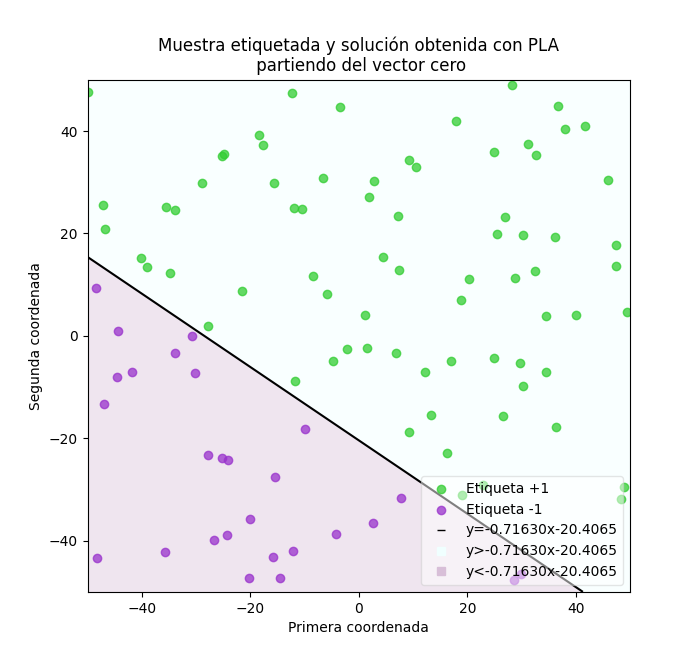
\includegraphics[width=77mm]{img/PLA_0.png}}
	\subfigure{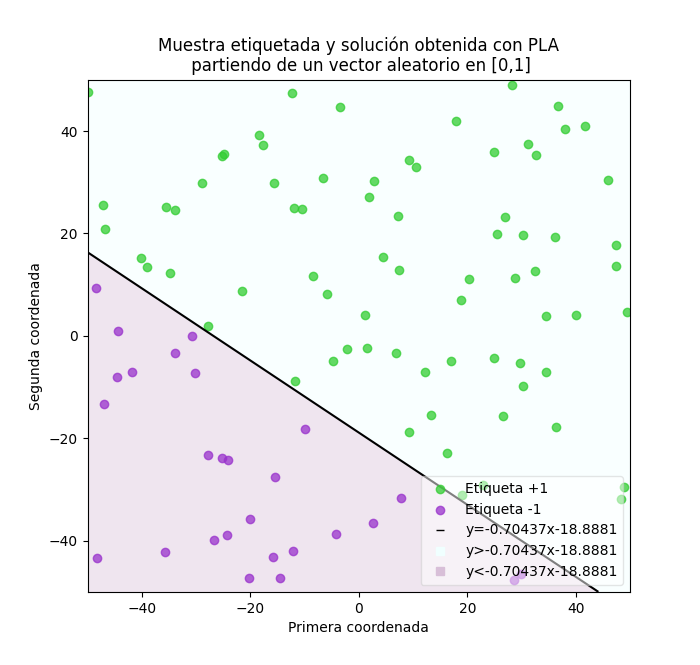
\includegraphics[width=77mm]{img/PLA_aleatorio.png}}
	\caption{Resultados PLA para una muestra sin ruido}
	\label{fig:PLA1}
\end{figure}

Podemos ver que en los dos casos las rectas obtenidas clasifican correctamente todos los puntos.

En la primera figura el vector de pesos es $ w=[661, 23.20241712, 32.39163606] $ y en la segunda\\ $w=[1024.85647306, 38.21852826, 54.25915726]$, correspondiente a la solución obtenida partiendo del vector aleatorio generado en la última repetición. 

Los coeficientes de la recta de clasificación en ambos casos han sido obtenidos igualando a 0 la función $h_w(x)=w^Tx$ y despejando la segunda característica con respecto a la primera como aparece en \href{https://stackoverflow.com/questions/42704698/logistic-regression-plotting-decision-boundary-from-theta}{https://stackoverflow.com/questions/42704698/logistic-regression-plotting-decision-boundary-from-theta}, de manera que $a=-w[1]/w[2]$ y $b=-w[0]/w[2]$. Notamos que dichos coeficientes son similares en las dos figuras, y están cercanos a $ a:  -0.6771584922002485,  b: -18.89022818933684 $, que son los parámetros de la recta real usada para etiquetar la muestra.  


El número de iteraciones del algoritmo necesarias para encontrar la solución partiendo del vector 0 es siempre el mismo, 75, ya que se trata de un algoritmo determinista: su funcionamiento es igual siempre que se parte de un mismo vector. En el caso en que partimos de vectores aleatorios, el número medio de iteraciones en las 10 repeticiones ha sido de 129.3. Es claro entonces que el punto de partida influye en la rapidez con la que converge el algoritmo, siendo el número de iteraciones que necesita para converger mayor o menor dependiendo del punto de partida. Este hecho se puede apreciar en la Tabla 1. Sin embargo, en el caso de muestras linealmente separables, el punto de partida no influye en la calidad de la solución obtenida, pues siempre se encuentra una solución óptima, como ya hemos comentado. 

\subsubsection{Apartado b)}

\textbf{Hacer lo mismo que antes usando ahora los datos del apartado 2b de la sección.1.
	¿Observa algún comportamiento diferente? En caso afirmativo diga cual y las
	razones para que ello ocurra.}

En este caso ejecutamos \lstinline|iteracionesPLA(x, etiquetas)| con la muestra y etiquetas generadas en el apartado 2b) de la sección 1, es decir, con la misma muestra que en el apartado anterior pero con ruido en las etiquetas. Los resultados se muestran en la siguiente tabla:

\begin{table}[htbp]
\begin{center}
	\begin{tabular}{|c|c|c|}
		\hline
		\textbf{Vector inicial de pesos} & \textbf{Número de iteraciones } & \textbf{Error} \\ \hline
		[0,0,0] & 10000 & 0.12 \\ \hline
		[ 0.16681, 0.4394, 0.16041 ] & 10000 & 0.13 \\ \hline
		[ 0.8792 , 0.47845, 0.39915 ] & 10000 & 0.19 \\ \hline
		[ 0.27547, 0.05164, 0.13871] & 10000 & 0.13 \\ \hline
		[ 0.77863 , 0.17805 , 0.58343 ] & 10000 & 0.12 \\ \hline
		[ 0.92812, 0.10766 , 0.45264 ] & 10000 & 0.17 \\ \hline
		[ 0.15599, 0.30421 , 0.76412] & 10000 & 0.18 \\ \hline
		[ 0.62692, 0.71109, 0.19346] & 10000 & 0.20 \\ \hline
		[ 0.06843, 0.87965 , 0.31984 ] & 10000 & 0.13 \\ \hline
		[ 0.60448 , 0.95521 , 0.41579 ] & 10000 & 0.13 \\ \hline
		[ 0.19589, 0.16602 , 0.6248 ] & 10000 & 0.14 \\ \hline
	\end{tabular}
	\label{}
	\caption{Resultados PLA para datos con ruido}
	\end{center}
\end{table}

Visualizamos las soluciones:

\begin{figure}[H]
	\centering    
	\subfigure{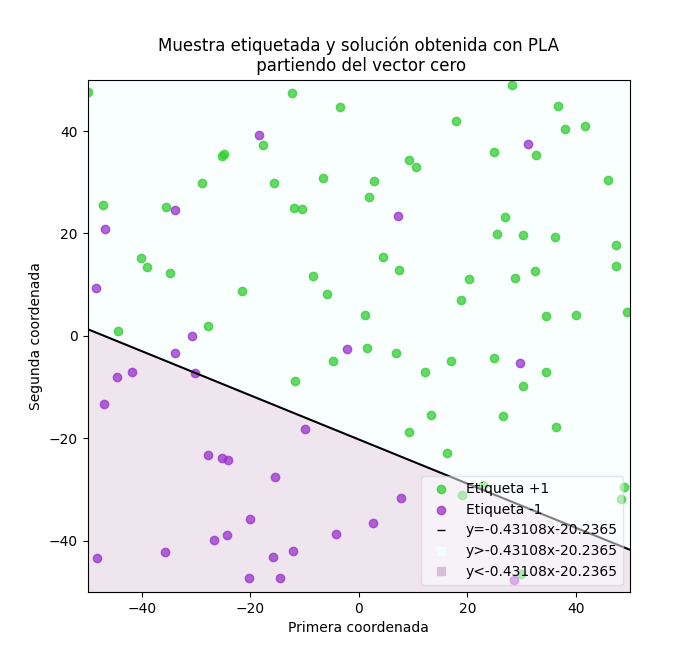
\includegraphics[width=77mm]{img/PLA_ruido1.png}}
	\subfigure{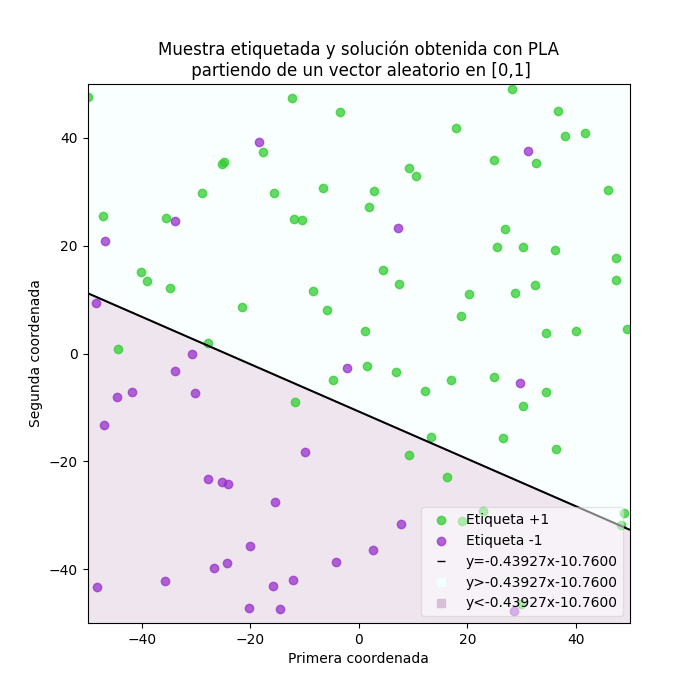
\includegraphics[width=77mm]{img/PLA_ruido2.png}}
	\caption{Resultados PLA para una muestra con ruido}
	\label{fig:PLA2}
\end{figure}

En la primera figura el vector de pesos es $ w=[298, 6.34801058, 14.72582576] $ y en la segunda\\ $w=[291.19589157,  11.8879214,   27.0626234 ]$, correspondiente a la solución obtenida partiendo del vector aleatorio generado en la última repetición. 

Al introducir ruido la muestra deja de ser linealmente separable, de modo que el algoritmo PLA no siempre encuentra la solución. En efecto, vemos en la Tabla 2 que el error de clasificación en la muestra no llega a ser 0, sino que da una media de 0.152 en las 10 repeticiones en que partimos de vectores aleatorios y es de 0.12 cuando se parte del vector nulo. 

En este caso el algoritmo para cuando alcanza el máximo número de iteraciones permitidas. Si no fijáramos un máximo número de iteraciones, el algoritmo no pararía nunca, pues, al no ser la muestra linealmente separable, en todas las épocas va a haber puntos mal clasificados, de modo que el criterio que hace que pare el algoritmo cuando todos los puntos están bien clasificados no se cumple nunca. Consideramos \lstinline|max_iter=1000|, tanto en este apartado como en el anterior, pues ya vimos en la Tabla 1 que, en caso de poder encontrar la solución, el algoritmo no necesita más de 300 iteraciones, con lo que 1000 es más que suficiente. 

Por otro lado, nos damos cuenta de que ahora el punto de partida sí influye en la calidad de la solución encontrada, el error varía según el vector de pesos inicial. Este hecho se puede apreciar tanto en la Tabla 2 como en las gráficas, en las que podemos ver que cuando se parte del vector 0 la solución encontrada es mejor que cuando se parte de otro vector aleatorio. 

En el caso de muestras no separables linealmente, este algoritmo devuelve el vector de pesos que se tiene en la última iteración, el cual no tiene por qué ser el mejor encontrado en todas las iteraciones. De ahí que el punto inicial influya en la calidad de la solución, pues la última iteración del algoritmo depende del vector inicial. 


\subsection{Ejercicio 2: Regresión Logística}
\textbf{En este ejercicio crearemos nuestra propia función
objetivo $ f $ (una probabilidad en este caso) y nuestro conjunto de datos $\mathcal{D}$ para ver cómo
funciona regresión logística. Supondremos por simplicidad que $ f $ es una probabilidad
con valores $ 0/1 $ y por tanto que la etiqueta $ y $ es una función determinista de $ x $.
}

\textbf{Consideremos $ d = 2 $ para que los datos sean visualizables, y sea $ \mathcal{X} = [0, 2] \times [0, 2] $ con
probabilidad uniforme de elegir cada $ x \in\mathcal{X} $ . Elegir una línea en el plano que pase por
 $ \mathcal{X} $ como la frontera entre $ f (x) = 1 $ (donde $ y $ toma valores +1) y $ f (x) = 0 $ (donde $ y $
toma valores -1).}

Usamos la función \lstinline|simula_unif| para generar una muestra uniforme de 100 puntos 2D en el cuadrado $ [0, 2] \times [0, 2] $. Con la función \lstinline|simula_recta| obtenemos los parámetros a y b de una recta que corte al cuadrado considerado, la cual usaremos como frontera de clasificación. Los parámetros aleatorios devueltos por esta función en mi caso han sido $a:  0.12435604777349397,  b: 1.1938712398529923$. 
A continuación, etiquetamos la muestra generada con \lstinline|etiquetar|, en este caso sin ruido en el etiquetado, tal y como hicimos en el apartado 2a) de la Sección 1. 

Veamos la muestra obtenida junto con la recta usada para la clasificación:

\begin{figure}[H]
	\centering
	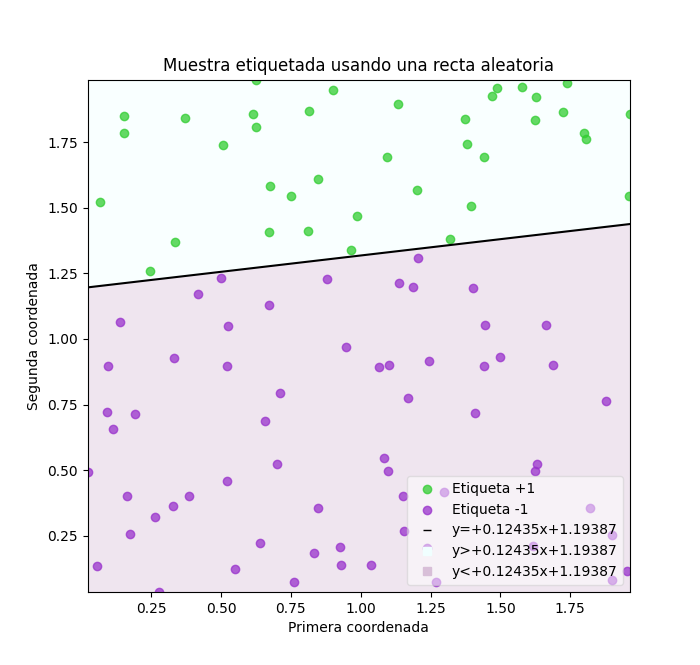
\includegraphics[width=0.6\linewidth]{img/RL1}
	\caption{}
	\label{fig:rl1}
\end{figure}



\subsubsection{EXPERIMENTO} 

\textbf{Seleccione $ N = 100 $ puntos aleatorios ${x_n } $ de  $ \mathcal{X} $ y evalúe las
respuestas $ {y_n } $ de todos ellos respecto de la frontera elegida. Ejecute Regresión
Logística para encontrar la función solución $ g $ y evalúe el
error $ E_{out} $ usando para ello una nueva muestra grande de datos $ (> 999) $. Repita el
experimento 100 veces, y}

\begin{itemize}
	\item \textbf{Calcule el valor de $ E_{out} $ medio para el tamaño nuestral $ N=100. $}
	\item \textbf{Calcule cúantas épocas tarda en converger en promedio RL para $ N=100 $ en las
	condiciones fijadas para su implementación.}
\end{itemize}


En primer lugar, implementamos el algoritmo de Gradiente Descendente Estocástico para Regresión Logística, en la función \lstinline|sgdLR(x,y, maxEpocas, lr)|, cuya implementación y detalles pueden encontrarse en el código de la práctica. 

En el caso de Regresión Logística, buscamos maximizar la verosimilitud de la muestra, es decir, la probabilidad de asignar a cada elemento de la muestra su verdadera etiqueta. Equivalentemente, se intenta minimizar el error
 $$E_{in}(w)=\frac{1}{N}\sum_{i=1}^{N}\log(1+e^{-y_iw^Tx_i})$$
donde $x_i$ es el punto i-ésimo de la muestra, $y_i$ es su etiqueta (+1 o -1), $ N $ es el tamaño de la muestra y $ w $ es el vector de pesos que determina una función lineal. Este error está definido en el código en \lstinline|Error_LR(w,x,y)|. 

El gradiente de este error en un punto $(x,y)$ es $-yx\sigma(-yw^Tx)$, siendo $\sigma(z)=\frac{1}{1-e^{-z}}$ la función sigmoide, que devuelve valores en $[0,1]$. Estas funciones se encuentran en el código en \lstinline|gradError(w, x, y)| y \lstinline|sigmoid(x)| respectivamente. 

El algoritmo SGD implementado considera un tamaño de batch de 1 (como se recomendó en clase) y una tasa de aprendizaje de \lstinline|lr|, que por defecto toma el valor 0.01. Lo que hace este algoritmo es crear un vector de índices permutados aleatoriamente, con tantos índices como elementos hay en el dataset, y recorrer uno a uno los datos, en el orden en el que aparecen sus índices en ese vector, actualizando el vector de pesos $w$ según la dirección del gradiente descendente del error en ese dato. Esto se repite durante un cierto número de épocas (número de pases completos por el dataset), determinado por el parámetro \lstinline|maxEpocas|, o hasta que la modificación del vector de pesos entre dos épocas consecutivas sea muy pequeña (concretamente se repite hasta que $\|w^{(t-1)}-w^{(t)}\|<0.01$, donde $\|.\|$ denota la norma euclídea y $t\in\{1,...,maxEpocas\}$ es la época). El parámetro \lstinline|maxEpocas| asegura que el algoritmo va a parar en algún momento, pues puede ocurrir que los datos no sean separables y nunca se cumpla la segunda condición de parada. Así, el pseudocódigo de este algoritmo es el siguiente:

\begin{lstlisting}[language=Python]
RL con SGD:
w <-- 0  # Vector inicial de pesos
cambio <-- True
epocas <-- 0
while cambio and epocas<max_epocas:
	w_anterior <-- w
	indices <-- shuffle({1,...,N}) #N es el tamanio del dataset
	for i in indices:
		w <-- w-lr*gradError(w,x,y)
	change <-- norm(w_anterior - w) > 0.01 #norm es la norma euclidea
	epocas <-- epocas + 1
return w, epocas

\end{lstlisting}

Lo ejecutamos sobre la muestra uniforme de 100 puntos creada, con su correspondiente etiquetado generado usando la recta aleatoria, y obtenemos la siguiente solución:

\begin{figure}[H]
	\centering
	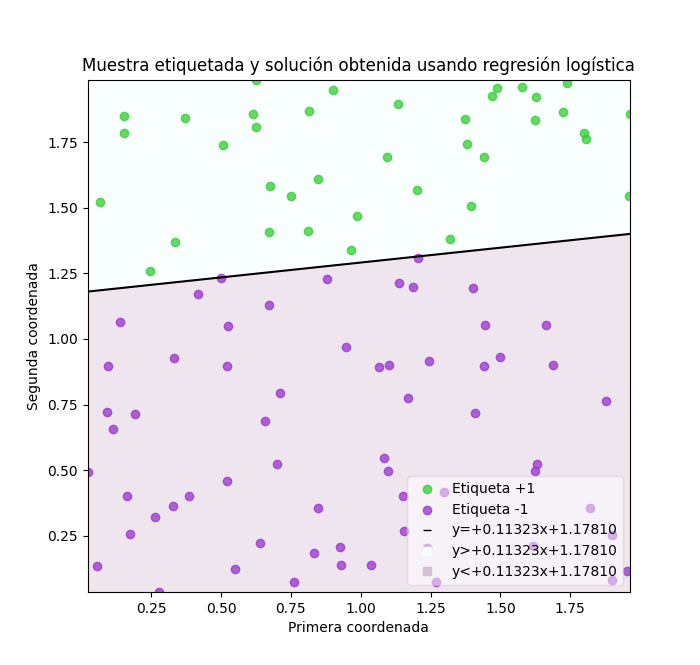
\includegraphics[width=0.6\linewidth]{img/RL2}
	\caption{}
	\label{fig:rl2}
\end{figure}

correspondiente a un vector de pesos $w= [-8.20520857, -0.78863086,  6.96472638]$. La solución encontrada mediante regresión logística es de la forma $g(x)=\sigma(w^Tx)$, con w ese vector, que asigna a x la probabilidad de que su etiqueta sea +1. Así, le asignamos a un punto la etiqueta +1 si dicha probabilidad es mayor o igual a $\frac{1}{2}$ y -1 en caso contrario.  Notamos que $$g(x)\geq \frac{1}{2}\Leftrightarrow w^Tx \geq 0 \Longleftrightarrow signo(w^Tx)=1$$ con lo que podemos usar para etiquetar la misma función que en clasificación lineal ($ y=signo(w^Tx) $). La recta de clasificación se corresponde con $g(x)=\frac{1}{2}$.

Podemos observar en la figura que la recta obtenida clasifica correctamente todos los puntos. De hecho, los parámetros a y b de la recta solución están muy cerca de los valores reales de dichos parámetros. 

El error de regresión logística en la muestra ($E_{in}$) es de 0.102679582, bastante bajo. Si además calculamos el error de clasificación utilizando la función \lstinline|Error(x,etiquetas,w)| (ya explicada), obtenemos que este es de 0, es decir, todos los puntos están bien clasificados, hecho que también se puede ver en la figura, como ya hemos dicho. 

Por otra parte, el algoritmo necesita 409 épocas para encontrar la solución. Hemos fijado un valor de \lstinline|maxEpocas=1000|, de modo que el algoritmo para mucho antes de llegar al máximo número de épocas permitido.

Generamos además un conjunto de test de 1500 datos 2D en el cuadrado $ [0, 2] \times [0, 2] $, usando la función \lstinline|simula_unif|, y los etiquetamos con nuestra recta aleatoria utilizando \lstinline|etiquetar|. Al calcular el error de regresión logística en este conjunto de test aleatorio (con \lstinline|Erro_LR|) obtenemos 0.11942972 y el error de clasificación es de 0.01333333. Ambos errores son ligeramente superiores a los obtenidos en la muestra, pero siguen siendo muy bajos.

Repetimos 100 veces el experimento, generando en cada iteración un conjunto nuevo de entrenamiento y de test, así como una nueva recta de clasificación. Calculamos la media del número de épocas que necesita el algoritmo para encontrar la solución en las 100 repeticiones, y los errores medios en la muestra y en test. Los resultados obtenidos son los siguientes:

\begin{itemize}
	\item \textbf{$ E_{in} $ medio (error de RL) tras 100 repeticiones del experimento:} 0.10946258366800354
	\item \textbf{ $E_{out}$ medio (error de RL) tras 100 repeticiones del experimento:} 0.11443781099649515
	\item \textbf{Proporción media de puntos mal clasificados en la muestra:} 0.01830000000000001
	\item \textbf{Proporción media de puntos mal clasificados en el conjunto de test:} 0.023733333333333335
	\item \textbf{Número de épocas promedio que necesita el algoritmo de RL para converger:} 416.93
	
\end{itemize}

Vemos ahora que el error de clasificación en la muestra no es 0, sino que es algo superior, de 0.0183, por lo que deducimos que en algunos casos el algoritmo de RL implementado no llega a encontrar una solución que clasifique correctamente todos los puntos de la muestra, como ocurría con PLA. Esto puede ser debido al margen de error de 0.01 que hemos considerado como criterio de parada del algoritmo (para cuando $\|w^{(t-1)}-w^{(t)}\|<0.01$), pues, aunque la modificación en el vector de pesos sea muy pequeña, puede que no sea nula, de manera que sigue habiendo puntos que la solución devuelta por el algoritmo clasifica mal. 

Todos los valores de los errores son pequeños, tanto en la muestra como en test, de manera que el algoritmo funciona bastante bien. Vemos que en el conjunto de test los errores son algo mayores que en el conjunto de entrenamiento, como era de esperar, pero aún así no son grandes, por lo que en general la solución encontrada por el algoritmo de RL generaliza bien fuera de la muestra. Por lo tanto, podemos decir que la regresión logística resuelve adecuadamente el problema de clasificación cuando los datos son separables. 

En cuanto al número medio de épocas, vemos que es de alrededor de 400, un número más elevado que el que necesitaba el algoritmo PLA, como vimos en el ejericicio 1 de esta sección. 

Podemos concluir entonces que este algoritmo de regresión logística es adecuado para problemas de clasificación en el caso de datos linealmente separables, pero ofrece soluciones de peor calidad que las de PLA y necesita más iteraciones para converger. 
 
\newpage
\section{BONUS: Clasificación de Dígitos Manuscritos}
\subsection{Ejercicio 1}

\textbf{Plantear un problema de clasificación binaria que considere el conjunto de entrenamiento
como datos de entrada para aprender la función $ g $.}

Tenemos un conjunto de dígitos manuscritos que queremos clasificar en dos clases correspondientes al dígito 4 y 8. Así, las etiquetas serán $y=+1$ para el dígito 8 e $y=-1$ para el dígito 4. Las características consideradas serán la intensidad promedio de gris, $x_1$, y la simetría respecto al eje vertical, $x_2$, de manera que un dato $x$ será un vector de la forma $x=(1,x_1,x_2)$. 

Queremos aprender una función $ g $ que asigne a cada punto $x$ su etiqueta $y$. Dicha función será\\ $g(x)=sign(w^Tx)$, para un cierto vector de pesos $w$. 

\subsection{Ejercicio 2}

\textbf{Usar un modelo de Regresión Lineal y aplicar PLA-Pocket como mejora.}

Aplicaremos el algoritmo de la Pseudo-inversa (explicado en la práctica 1) y PLA-Pocket para intentar aprender el vector de pesos $ w $ que determina a la función $ g_w(x) $ que separa los datos en las dos clases. 

El algoritmo PLA-Pocket es una modificación del algoritmo PLA, estudiado en el ejercicio 1 de la Sección 2. Este nuevo algoritmo calcula tras cada época el error de clasificación proporcionado por la solución asociada al vector de pesos obtenido en esa época, guardando el vector de pesos que ha ocasionado el menor  error en la muestra hasta ese momento. El algoritmo para tras un determinado número de iteraciones, especificado por el programador, devolviendo el vector $w$ con menor error encontrado tras ese número de iteraciones (consideramos una iteración como una época). La función \lstinline|Pocket(datos, label, maxIter, vini)| implementa este algoritmo. Como está implementado, además del vector de pesos, el algoritmo almacena y devuelve el menor error obtenido, asociado al vector de pesos guardado (para no tener que calcula el error de nuevo fuera de esta función). El pseudo-código de PLA-Pocket queda como sigue:

\begin{lstlisting}[language=Python]
PLA-Pocket:
w <-- vini  # Vector inicial de pesos
mejor_w <-- w
mejor_error <-- Error(datos,label,mejor_w)
for i in {1,...,maxIter}:
	for x in datos:
		if signo(w.T*x)!= y: # Etiqueta asociada al punto x
			w <-- w + x*y
	error <-- Error(datos,label,w)
	if error < mejor_error:
		mejor_error <-- error
		mejor_w <-- w
return mejor_w, mejor_error

\end{lstlisting}

Ejecutamos el algoritmo de la pseudo-inversa sobre el conjunto de datos de entrenamiento y a continuación corremos PLA-Pocket (con \lstinline|maxIter=1000|, como venimos haciendo hasta ahora) con el vector de pesos obtenido como punto de partida. Con la pseudo-inversa obtenemos una expresión cerrada para el vector de pesos w, que probablemente estará cerca de la solución del problema de clasificación, pues al minimizar el error de regresión también se minimiza el de clasificación. Es muy probable que \(sign(w^Tx_n)\) coincida con la etiqueta correcta \(y_n=\pm 1\). El algoritmo PLA-Pocket se encargará entonces de mejorar la solución, minimizando el error de clasificación. 
\newpage
\subsubsection{Apartado a)}
\textbf{Generar gráficos separados (en color) de los datos de entrenamiento y test junto con
la función estimada.}

La solución obtenida con el algoritmo de la pseudo-inversa ha sido $w=[-0.50676351,  8.25119739,  0.44464113]$. Mostramos la solución gráficamente junto con los datos de entrenamiento y los de test, usando la función \lstinline|plotEtiquetado|:

\begin{figure}[H]
	\centering    
	\subfigure{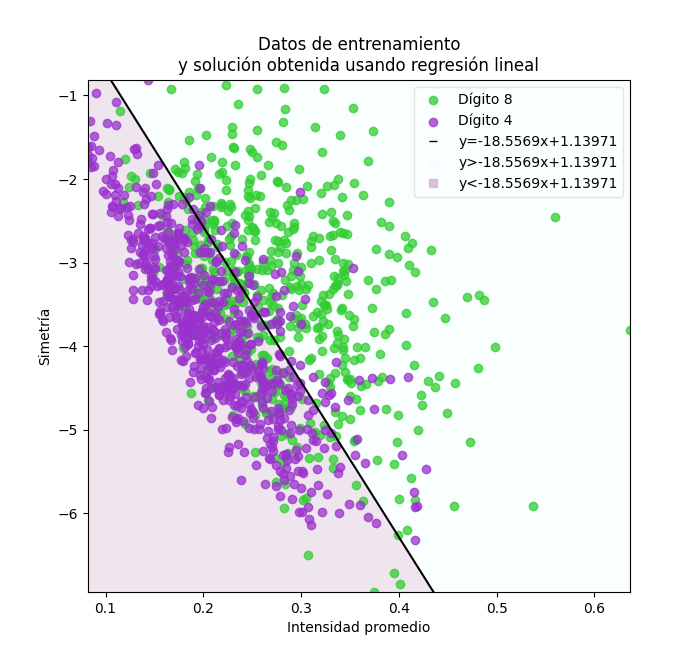
\includegraphics[width=77mm]{img/pseudoinversa.png}}
	\subfigure{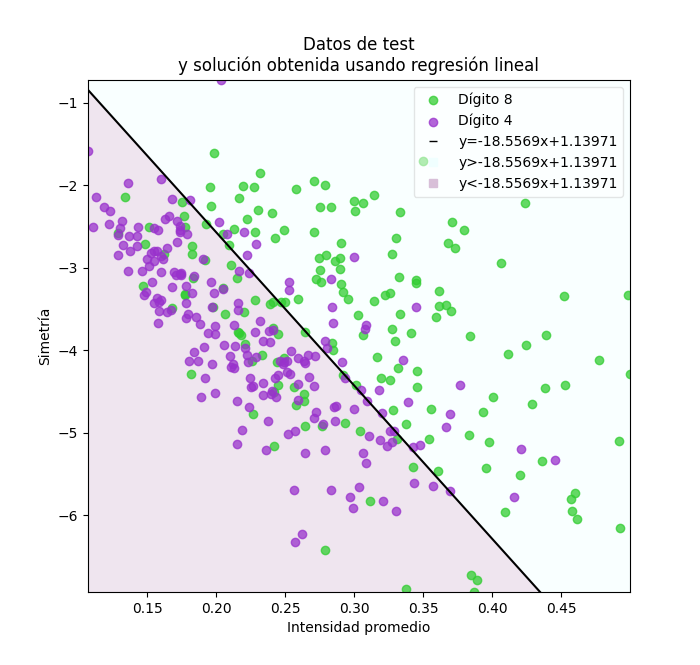
\includegraphics[width=77mm]{img/pseudoinversa2.png}}
	\caption{Resultados Pseudo-inversa}
	\label{fig:pseudo-inversa}
\end{figure}

PLA-Pocket mejora entonces la solución, proporcionando un vector de pesos\\ $w=[-6.50676351, 94.33278003,  4.88432863]$.

\begin{figure}[H]
	\centering    
	\subfigure{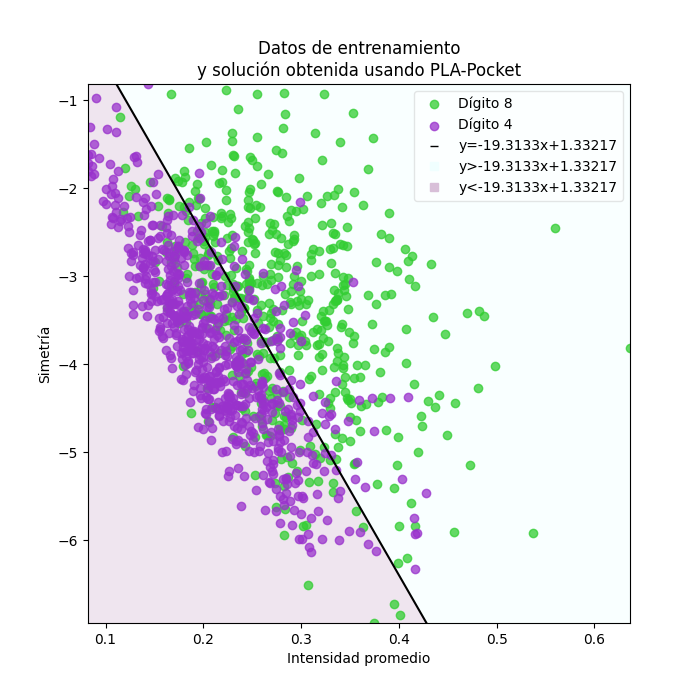
\includegraphics[width=77mm]{img/pocket1.png}}
	\subfigure{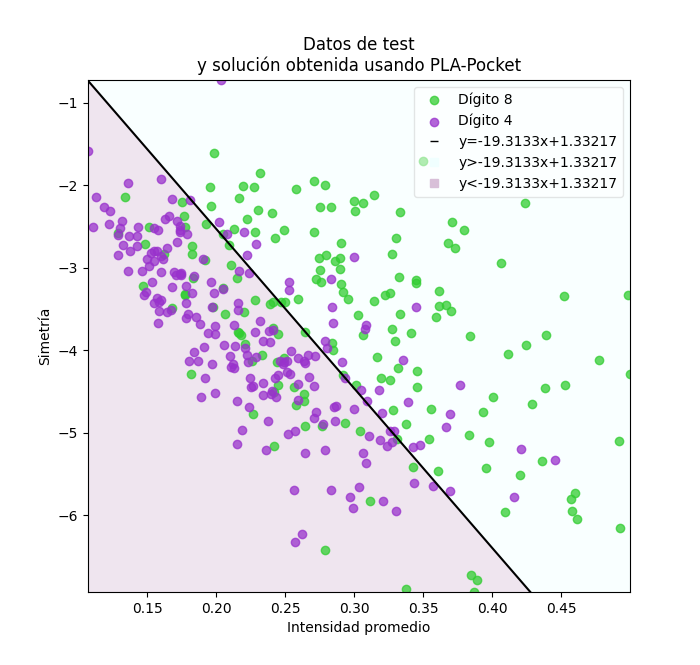
\includegraphics[width=77mm]{img/pocket2.png}}
	\caption{Resultados de PLA-Pocket}
	\label{fig:pocket}
\end{figure}

Observamos que ambas soluciones son bastante parecidas y clasifican correctamente una gran cantidad de los puntos. 

\subsubsection{Apartado b)}
\textbf{Calcular $ E_{in} $ y $ E_{test} $ (error sobre los datos de test).}

No podemos concluir nada preciso simplemente viendo las figuras anteriores, por lo que calculamos los errores de clasificación en ambos casos tanto en la muestra como en el conjunto de test, y los resultados obtenidos han sido los siguientes:

\textbf{Algoritmo de la pseudo-inversa}

\begin{itemize}
	\item $E_{in}$: 0.22780569514237856
	\item $E_{test}$:  0.25136612021857924	
\end{itemize}

\textbf{Algoritmo PLA-Pocket}
\begin{itemize}
	\item $E_{in}:$ 0.22529313232830822
	\item $E_{test}:$ 0.2540983606557377
\end{itemize}

Vemos que efectivamente el algoritmo de PLA-Pocket mejora la solución proporcionada por regresión lineal, ya que presenta un error de clasificación en la muestra ligeramente menor.  Sin embargo, el error en el conjunto de test es algo superior en la solución que nos da PLA-Pocket que en la obtenida por la pseudo-inversa. Esto puede ser debido a que la primera se ajusta más a los datos de la muestra, ocasionando una peor generalización fuera de la misma.

Nos damos cuenta, además, de que la solución que proporciona la regresión lineal resuelve muy bien el problema de clasificación en este caso, pues el algoritmo Pocket consigue mejorar sólo un poco la misma, hecho que se aprecia tanto en los errores obtenidos como en las figuras del apartado anterior, donde vemos que las fronteras de clasificación son muy similares. De hecho, la solución que nos da regresión lineal generaliza fuera de la muestra mejor que la que nos da Pocket.

\subsubsection{Apartado c)}

\textbf{Obtener cotas sobre el verdadero valor de $E_{out}$ . Pueden calcularse dos cotas una
basada en $E_{in}$ y otra basada en $E_{test}$ . Usar una tolerancia $\delta = 0.05$. ¿Qué cota es
mejor?}

Usando la desigualdad de Hoeffding y la dimensión de VC, tenemos que una cota para $E_{out}$ es:
$$E_{out}(h)\leq E_{in}(h) + \sqrt{\frac{8}{N}\log\frac{4((2N)^{d_{VC}}+1)}{\delta}}$$
donde N es el número de datos de la muestra, $d_{VC}$ es la dimesión de VC de la clase de funciones considerada y $\delta$ es la tolerancia (la desigualdad se cumple con probablidad de al menos $1-\delta$).

En nuestro caso estamos tomando como clase de funciones la clase del perceptron 2D, por lo que sabemos que $d_{VC}=3$. Además, tenemos que $N=1194$ en el conjunto de entrenamiento. Por lo tanto, la cota que obtenemos para $E_{out}$ basada en $E_{in}$ es la siguiente:

$$E_{out}(h)\leq E_{in}(h) + \sqrt{\frac{8}{1194}\log\frac{4((2\times 1194)^{3}+1)}{0.05}}= 0.22529313232830822 + 0.4309365055 = 0.6562296378 $$ $$\Rightarrow E_{out} \leq 0.6562296378 $$

con probabilidad mayor o igual a 0.95.

La desigualdad de Hoeffding nos permite obtener una cota basada en el error obtenido en un conjunto de test ($E_{test}$):

$$E_{out}(g)\leq E_{test}(g) + \sqrt{\frac{1}{2N}\log\frac{2}{\delta}} = E_{test}(g) + \sqrt{\frac{1}{2\times366}\log\frac{2}{0.05}}=0.2540983606557377 + 0.07098910343=0.3250874641$$ $$\Rightarrow E_{out} \leq 0.3250874641$$

con probablidad mayor o igual a 0.95. Hemos usado que para nuestro conjunto de test $N=366$, y $\delta=0.05$. 

Cabe notar que ahora la hipótesis $g$ está fija, ya la hemos elegido, no hay infinitas funciones como en el caso anterior. Esto hace que la cota obtenida usando $E_{test}$ sea bastante mejor que la obtenida usando $E_{in}$, pues como vemos es mucho menor. Además, el hecho de usar datos que no se han utilizado para el aprendizaje también hace que esta cota sea más representativa (es independiente de los datos de entrenamiento).


\end{document}